
\part{Apêndice}


\begin{center}
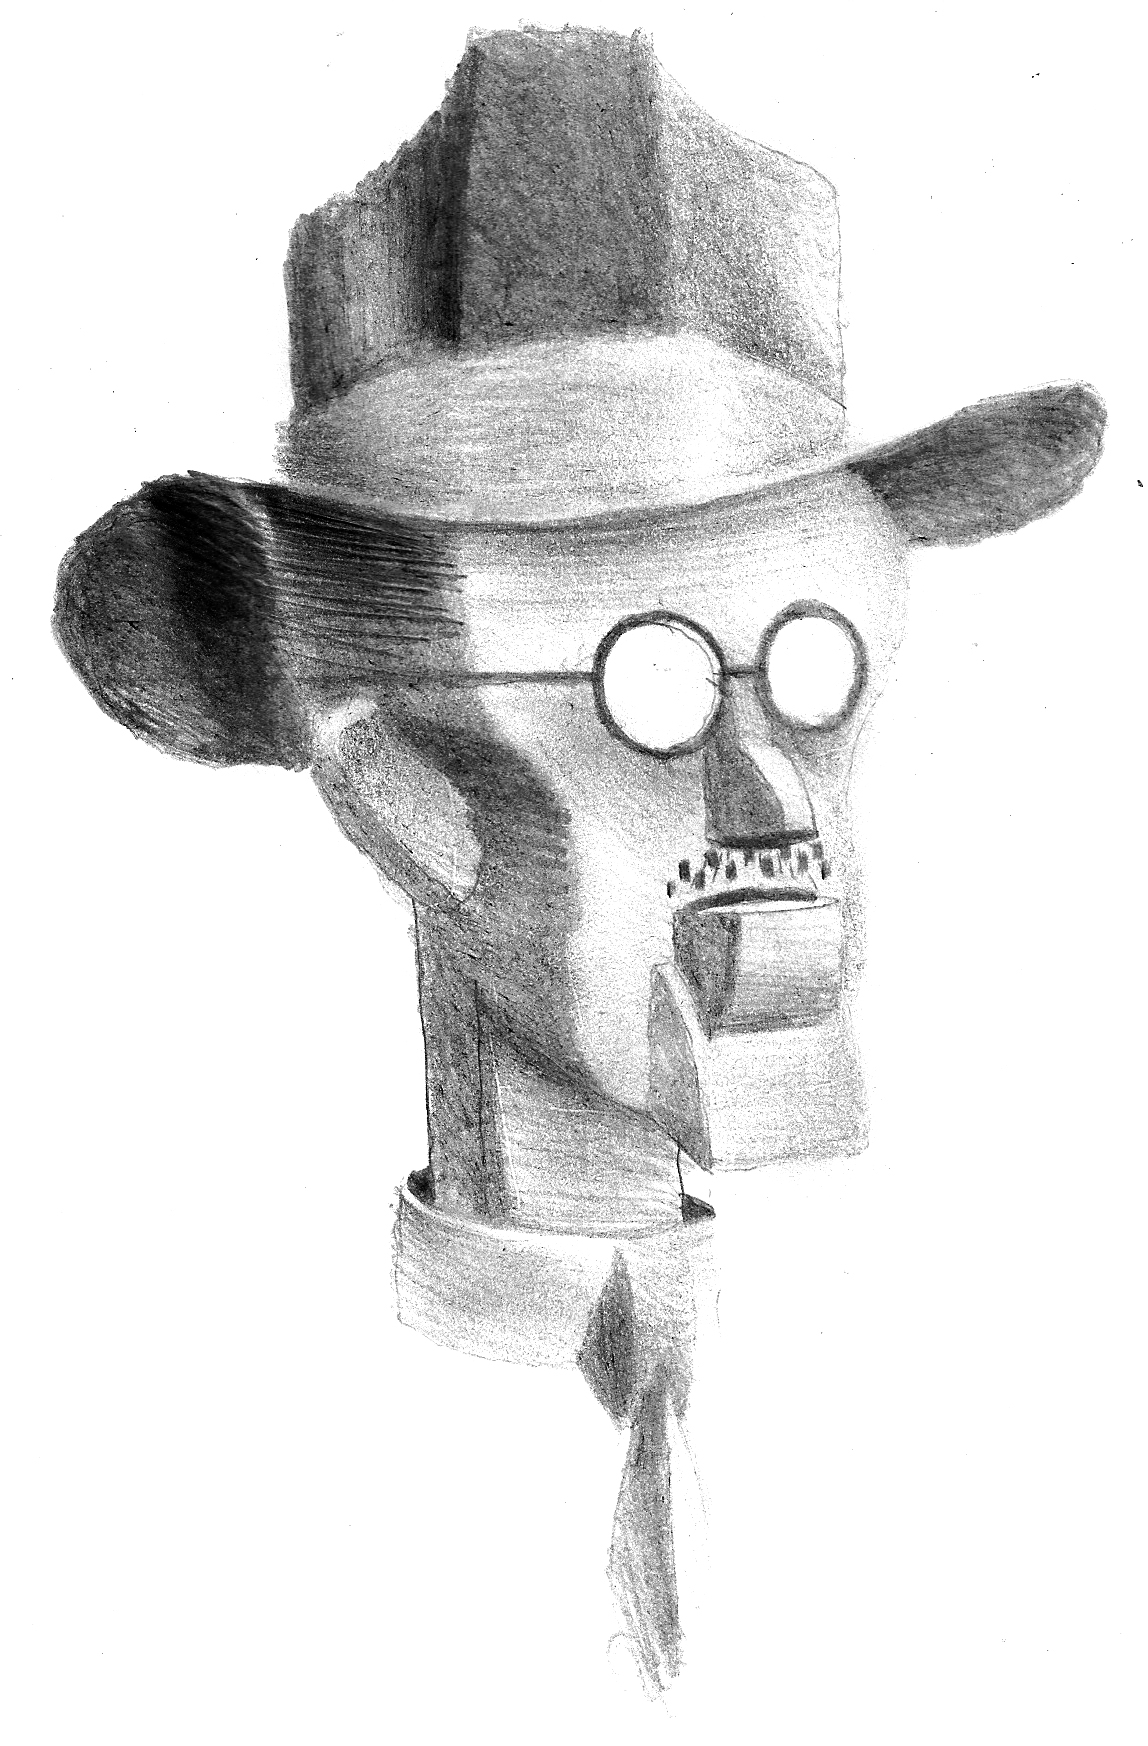
\includegraphics[width=.6\textwidth]{./joyce3.jpg}
\end{center}


\chapterspecial{O retrato da Irlanda}{}{Beatriz Kopschitz Bastos}

\markboth{O retrato da Irlanda}{Beatriz Kopschitz Bastos}

\noindent\textsc{O nacionalismo} irlandês, em suas três vertentes ---  revolucionário,
parlamentar e cultural --- contra o qual tanto James Joyce quanto Stephen
Dedalus se revoltam, foi característico de períodos anteriores e
contemporâneos à publicação do \textit{Retrato} e é um dos principais
componentes históricos que permeia o romance. Uma narrativa breve da
história que antecedeu, gerou e constituiu esse nacionalismo auxilia,
portanto, o leitor a compreender as muitas alusões presentes no
romance. 

Os primeiros habitantes da Irlanda, caçadores, devem ter chegado antes
do ano 6000~a.C. Ao longo dos séculos, desenvolveram uma cultura rural,
cujos dolmens remanescentes podem ser vistos ainda hoje. Com o passar
do tempo, ocorreram outras levas de invasões, mas pode"-se dizer que a
verdadeira história da Irlanda começa com a chegada dos celtas, em
torno do ano 600~a.C. Apesar de sua derrota por Roma no continente e na
Inglaterra, os povos celtas da Irlanda permaneceram intactos, mesmo
depois da queda de Roma, e a civilização celta, ainda hoje, é parte
importante da cultura nacional irlandesa.

A primeira grande mudança cultural na Irlanda ocorreu com a vinda de são
Patrício e do cristianismo no século \textsc{v}. Muitas lendas se desenvolveram
em torno da figura de são Patrício, a maioria delas sem fundamento
histórico, mas o cristianismo e a religião católica passaram a ser
parte fundamental da história e da cultura da Irlanda para sempre,
sendo que a grande ação transformadora trazida pela da Igreja Católica
talvez seja a introdução da língua escrita no país. 

 No século \textsc{viii} ocorreu a invasão viking, em consequência da qual muitos
dos mosteiros cristãos foram destruídos e muitas das principais cidades
de hoje, como Dublin e Cork, fundadas. Os vikings foram derrotados sob
a liderança de Brian Boru, vitória que muitos consideram ter trazido
alguma noção de unidade política à Irlanda, até então praticamente
inexistente. A unidade, porém, ainda muito frágil, permitiu que a
primeira invasão inglesa, no século \textsc{xii}, fosse possível e fácil. Os
guerreiros invasores, superiores em armas e exércitos, construíram
castelos e fortalezas por todo o território. A Irlanda tornou"-se, em
grande parte, uma colônia anglo"-normanda, ainda que a invasão não se
tenha dado de forma planejada e sistematizada. Aos poucos, a
convivência dos diferentes povos passou a ser pacífica e integrada. O
leste era praticamente anglo"-normando, enquanto o oeste permanecia
predominantemente gaélico. Estabeleceu"-se, assim, uma aristocracia
anglo"-irlandesa local.

Foi somente a partir do século \textsc{xvi}, principalmente com Henrique \textsc{viii} e a
Reforma Protestante, que a Inglaterra passou realmente a se importar
com a Irlanda, com o poder da aristocracia anglo"-irlandesa e com a
predominância católica. Elizabeth \textsc{i} teve um papel mais ativo na questão
irlandesa, enviando emissários a fim de tentar conter as incipientes
rebeliões, que aconteciam principalmente em Ulster, no norte da
Irlanda. A aristocracia gaélica local foi derrotada e abandonou as
terras de Ulster, possibilitando a expulsão dos irlandeses, o confisco
de terras e o repovoamento da região por ingleses protestantes.

O terror e o derramamento de sangue recrudesceram, mais tarde, no século
\textsc{xvii}, após a derrota de Carlos \textsc{i}, filho de Jaime \textsc{i} e a vitória de
Oliver Cromwell na guerra civil inglesa. A Irlanda católica ficara fiel
à coroa inglesa durante a guerra civil e o acerto de contas de Cromwell
foi implacável. Católicos foram massacrados em Drogheda e Wexford, em
retaliação às atrocidades cometidas contra protestantes em Ulster e, em
todo o país, pessoas foram mortas e vilas e igrejas destruídas. As
terras dos católicos foram confiscadas e, como se dera no norte,
começou a derrocada e emigração da aristocracia gaélica no sul. Os
camponeses irlandeses, em sua maioria de religião católica e falantes
de gaélico, passaram a ter novos senhores protestantes ingleses ou
escoceses. Estabelecia"-se, assim, o domínio da chamada
\textit{Protestant Ascendancy}, a classe alta protestante, que duraria
até o fim do século \textsc{xix}.  

A Revolução Gloriosa na Inglaterra culminou na queda de Jaime \textsc{ii}, último
rei inglês católico, que se refugia na Irlanda mas é derrotado por
Guilherme \textsc{iii} na batalha de Boyne em 1690. A vitória do rei protestante
leva, após alguma resistência, a uma fuga em massa das tropas
irlandesas, deixando a Irlanda totalmente subjugada pelo domínio inglês
protestante e cada vez mais uma colônia da Inglaterra.

A partir de então medidas drásticas de exclusão e punição, as chamadas
“leis penais”, passaram a ser infligidas aos católicos, que, por
exemplo, foram excluídos do parlamento, não podiam participar do
governo, do exército, votar ou ter escolas. Os católicos empobreciam,
enquanto a aristocracia anglo"-irlandesa protestante prosperava cada vez
mais. Naquele momento, a revolução e a organização política estavam
fora de cogitação para a população de camponeses irlandeses católicos.
Surgia, entretanto, uma classe média de comerciantes e intelectuais
católicos e, principalmente, protestantes, que crescia em bens e poder.
Alguns dos líderes dessa classe, entusiasmados com os ideais da
Revolução Francesa e com a guerra pela independência americana, e
insatisfeitos com a situação social e comercial imposta à Irlanda,
começaram a fomentar ideias de reformas sociais e emancipação. 

O anseio revolucionário concretizou"-se em alguns dos momentos históricos
mencionados anteriormente. O primeiro deles, 1798, foi liderado por
Theolbald Wolfe Tone, advogado protestante que fundou um braço do grupo
então chamado \textit{United Irishmen}, os Irlandeses Unidos,
em Dublin. Wolfe Tone pretendia a obtenção do alívio das “leis penais”
para os católicos e a independência. Sua principal atuação foi
trabalhar como representante dos radicais irlandeses na obtenção de
apoio francês, com focos de rebelião em Wexford e Ulster. No entanto,
quando finalmente os franceses desembarcaram na Irlanda 1798, ele foram
rapidamente derrotados. Wolfe Tone foi preso, julgado e condenado,
escapando da execução somente por suicídio. Após a rebelião, houve
revanche e opressão: morte, tortura, prisões e deportações.
Paradoxalmente, a consequência direta da rebelião de 1798 foi não a
independência, mas o estabelecimento do Reino Unido da Grã"-Bretanha e
Irlanda em 1801.  

Nos princípios revolucionários de Wolfe Tone surgia, entretanto, um
nacionalismo que culpava a Inglaterra por todos os problemas da Irlanda
e recorria à luta armada e ao derramamento de sangue como forma
primordial de obter a independência, princípios dos quais os
revolucionários futuros se considerariam herdeiros. 

Em repúdio à União de 1801, seguiu"-se em Dublin, sob o comando de Robert
Emmet em 1803, uma tentativa de levante que deveria coincidir com a
possível invasão da Inglaterra por Napoleão. O levante fracassou, e a
decisão dos insurgentes de atacar o Castelo de Dublin e assassinar Lord
Kilwarden, aparentemente contra a vontade de Emmet, levou à sua fuga,
mas ele acabou preso, julgado, condenado e executado. O tratamento
lendário para sempre dado a Emmet na literatura e na historiografia
nacionalista deve muito a seu discurso, dotado de fortíssimo apelo
emocional, proferido antes de ser enforcado. 

O espírito das palavras de Emmet gerou a sensibilidade de revolucionário
futuros, como Patrick Pearse: o sentimento de que o fracasso glorioso e
o martírio seriam, um dia, justificados e redimidos pela Irlanda
liberta. Assim, com a execução de Emmet, engrossavam"-se as fileiras dos
mártires da causa nacionalista a serem cultuados pelos defensores de um
nacionalismo revolucionário e romântico que predominou no século \textsc{xix} e
parte do século \textsc{xx}. 

Além do nacionalismo revolucionário que usava da luta armada, merece
também atenção a agitação de massas como forma de resistência e luta no
século \textsc{xix}. Destaca"-se a figura do advogado Daniel O’Connell, que
liderou diversas manifestações de multidões, principalmente católicas
como ele. O’Connell foi, de fato, a figura política dominante da
Irlanda pós"-União. Por meio de sua atuação, os católicos obtiveram a
Emancipação em 1829, que os livrou das últimas “leis penais” em vigor.
Tendo agora direito a voto, os católicos elegeram o próprio O’Connell
para o Parlamento. Após a vitória obtida com a Emancipação, O’Connell
passou a liderar as massas em campanha pela revogação da União. Em
1844, foi preso e seu movimento fracassou.

No movimento pela revogação da União, O’Connell contou inicialmente com
a colaboração de jovens nacionalistas, membros do grupo \textit{Young
Ireland}, a Irlanda Jovem: Thomas Davis, Charles Gavan Duffy,
John Blake Dillon, John Mitchel e James Fintan Lalor. O’Connell e os
membros da \textit{Young Ireland} acabaram por desentender"-se
principalmente quanto aos métodos para obter da revogação da Lei de
União, sendo as propostas dos jovens nacionalistas mais radicais do que
as de O’Connell. Considera"-se que com esse grupo nasceu um nacionalismo
romântico, que tinha a idéia de \textit{Irishness} acima de qualquer
outro princípio, a língua e a cultura como centrais para o conceito de
identidade nacional e que defendia a luta armada. Considera"-se também
que, como o nacionalismo de Wolfe Tone, o nacionalismo dos membros da
\textit{Young Ireland} caracterizava"-se por ser inclusivo e não
sectário. O movimento se desintegrou na tentativa fracassada de um
levante em 1848.

Cabe aqui observar que a grande catástrofe da primeira metade do século
\textsc{xix} foi sem dúvida a Grande Fome, que acometeu a Irlanda de 1845 a
1852. A devastação das plantações de batata causada por uma praga
deixou sem alimento mais da metade da população e desmantelou a
economia do país. Como consequência, estima"-se que um milhão de pessoas
tenha morrido, enquanto meio milhão tenha emigrado, ou seja, que a
população tenha caído de oito milhões para seis milhões e meio. A Fome
tornou"-se um componente central no processo de autorreconhecimento do
povo irlandês e, para os nacionalistas, foi prova do fracasso da União.

Na Irlanda pós"-Fome, destaca"-se o movimento pela reforma agrária,
principalmente por meio da atuação da \textit{Land League}, a Liga pela
Terra, liderada por Charles Stewart Parnell e Michael Davitt. Embora
fosse um movimento basicamente constitucional e de campanhas de massa
pacíficas, ocorreram muitas vezes rebeliões violentas nas áreas rurais,
no que ficou conhecido como \textit{land war}, a guerra pela
terra.  Aliava"-se, assim, ao movimento nacionalista um
movimento de reforma agrária, que defendia a criação de uma classe de
proprietários rurais camponeses.  

Considerando, por enquanto, principalmente o lado revolucionário do
nacionalismo, destaca"-se nesse período e no início do século \textsc{xx} a
formação de sociedades e organizações que conspiravam e trabalhavam em
prol da revolução armada. A \textit{Irish Republican Brotherhood}
incluía membros conhecidos como Fenianos, cujo nome foi tomado de um
ciclo de histórias medievais, o \textit{Fenian Cycle}, que descrevia as
aventuras do herói mítico, Fionn MacCumhail, de seu filho, Oisin, e dos
guerreiros Fianna. O \textit{Sinn Fein}, que significa
``nós mesmos'', em gaélico, era uma organização dominada por Arthur
Griffith, proveniente da fusão de vários grupos nacionalistas. Griffith
pretendia uma organização basicamente propagandista, que convencesse
outros nacionalistas de sua teoria de monarquia dualista, nos moldes do
império Austro"-Húngaro.  

Junto ao movimento nacionalista, fortalecia"-se também o movimento de
trabalhadores industriais e urbanos. Dois dos principais líderes do
movimento trabalhista foram James Connolly e Philip Larkin, que atuavam
no \textit{Irish Transport and} \textit{General Workers’ Union}, o
sindicato de trabalhadores dos transportes e dos trabalhadores em geral. O movimento
socialista gerou passeatas, prisões, brutalidade e greves e a
consequência de uma greve geral em 1913 foi a formação de um corpo de
voluntários armados, o \textit{Irish Citizen Army}, liderado por James
Connolly.

O momento culminante da ação de todos esses grupos foi o Levante de
Páscoa de 1916. O Levante ocorreu entre a segunda"-feira, 24 de
abril e o sábado, 29 de abril, na Semana da Páscoa. Os rebeldes
ocuparam diversos prédios importantes na área central de Dublin e
transformaram os a Agência Central dos Correios, o \textit{General Post
Office}, na O’Connell Street, em seu quartel general. Ali, Patrick
Pearse leu uma proclamação estabelecendo um governo provisório da
República da Irlanda. 

Suprimido o levante, mais de duas mil pessoas foram detidas, noventa
prisioneiros condenados à morte e quinze deles executados --- os líderes
e assinantes da Proclamação. Embora o levante não tenha contado
inicialmente com o apoio popular, as execuções rapidamente contribuíram
para a mitificação e adoração dos heróis de 1916 e a ebulição da causa
nacionalista, rejeitada por Joyce. 

Ao lado do nacionalismo revolucionário que favorecia a rebelião armada e
a agitação de massas e talvez obtendo mais avanços que as lutas armadas
e a guerrilha, desenvolveu"-se ao longo dos anos uma luta parlamentar e
gradual pela independência, em que se destaca o papel de Charles Stewart
Parnell.  

Embora um Parlamento Irlandês tivesse existido desde a Idade Média, sua
importância era pequena devido à subordinação ao Parlamento Inglês em
Westminster. Com a atuação e sob a liderança de Henry Grattan, apoiado
pelos voluntários do século \textsc{xviii}, e com o prestígio da
\textit{Ascendancy} protestante, o Parlamento Irlandês obteve total
independência no sentido de legislar soberanamente sobre a Irlanda. O
Parlamento de Grattan, como ficou conhecido, obteve medidas de alívio
das “leis penais”, bem como alívio de restrições comerciais. Além
disso, pretendia a revogação da União e a Emancipação dos católicos. A
Revolução de 1798, entretanto, somada à inabilidade do Parlamento
Irlandês de reformar sua estrutura de representação, admitindo a
inclusão de católicos, acabou por gerar a extinção do Parlamento de
Grattan. Os irlandeses passaram então a exercer sua representação
parlamentar somente em Westminster.

Durante muito tempo, a grande dificuldade irlandesa no Parlamento inglês
foi alcançar a formação de um partido único que lutasse pelas mesmas
causas e pudesse avançar na obtenção de concessões para a Irlanda.
Daniel O’Connell havia conseguido alguma união nas décadas de 1830 e
1840, baseada, entretanto, principalmente em seu carisma e em alianças
pessoais. Quase todas as outras tentativas de unificação, todavia,
giravam em torno de questões religiosas ou agrárias, sem grande
participação das massas. 

 A formação de um Partido Parlamentar Irlandês e a aliança dos
movimentos populares com a pressão parlamentar encontraram expressão na
figura de Charles Stewart Parnell. Protestante, líder, porém, também
dos católicos, Parnell organizou a formação do Partido Parlamentar
Irlandês, presidiu a \textit{National Land League} e, principalmente,
concentrou"-se na luta parlamentar para tornar realidade a questão do
autogoverno pela \textit{Home Rule} ---, revogação da União e
instauração de um Parlamento independente. Em 1889, a realização dessa
antiga aspiração estava praticamente em suas mãos. No entanto, o
envolvimento amoroso de Parnell com Kitty O’Shea, casada com o Capitão
William O’Shea, veio a público no mesmo ano e, transformado em
escândalo nacional, dividiu a política e a opinião pública e acabou por
trazer a derrocada política de Parnell e de seu partido. Parnell
faleceu dois anos depois.

O Partido Parlamentar Irlandês reunificou"-se somente em 1900, sob a
liderança de John Redmond. O Partido de Redmond  pretendia ser
predominantemente católico, sem ser subserviente à Igreja, e
genuinamente nacionalista, sem ser sectário. A atuação de Redmond
conseguiu avanços na obtenção da \textit{Home Rule}, tendo
sido aprovado o \textit{Home Rule Act}, em 1914. A aprovação
final da lei, entretanto, ficaria vinculada ao término da guerra e à
solução de questões em Ulster. Havia a impressão de que um longo
capítulo na história chegava ao fim. Tal impressão, entretanto, não
poderia estar mais longe da realidade, pois a carreira e o partido de
Redmond foram desmantelados após o levante de 1916. 

Aliada e algumas vezes em choque com o nacionalismo político, crescia,
no fim do século \textsc{xix}, uma outra força nacionalista. Assim como em toda
a Europa do século \textsc{xix}, o sentido político de nacionalidade entre povos
oprimidos ou subjugados foi, então, acompanhado de um nacionalismo
cultural que valorizava a língua, a literatura, o passado e a história.
Assim, o chamado nacionalismo cultural, que governou grande parte da
atividade cultural e intelectual da Irlanda entre aproximadamente 1880
e 1930, era uma força distinta, mas intimamente ligada ao nacionalismo
político.  

Embora um interesse pelo passado e pela cultura já estivesse em curso
desde o início do século \textsc{xix}, por meio de sociedades de especialistas e
intelectuais, todas as iniciativas eram, de alguma forma, limitadas.
Uma associação de outra natureza, \textit{The Gaelic Athletic
Association}, a Asssociação Atlética Gaélica, conseguiu maior adesão e
disseminação popular. Seus membros, em todo o país, mantinham estreitas
relações com as alas mais radicais do nacionalismo político e
rejeitavam todo tipo de esporte estrangeiro, principalmente inglês,
determinando um antianglicanismo sectário e assim contribuindo para o
renascimento de um novo espírito nacional.

A base intelectual ou cultural do nacionalismo viria por meio de outros
três movimentos, que, em conjunto, constituíram o \textit{Revival}, o
Renascimento Irlandês: o movimento pela língua, com a \textit{Gaelic
League}, a Liga Gaélica, o Movimento Literário Irlandês e o Movimento
Dramático Irlandês.

A atividade da \textit{Gaelic League}, fundada em 1893, foi sem dúvida
um dos principais fatores para o surgimento de um novo sentido de
nacionalidade. Seus objetivos eram a preservação do irlandês como
língua nacional, a extensão de seu uso como língua falada e o estudo e
publicação de literatura gaélica, bem como o incentivo à produção de
literatura em irlandês. Seus ideais projetavam uma união popular em
torno da questão da língua, rompendo barreiras de classe, gênero e
religião. Em termos práticos, a Liga obteve a introdução do ensino de
irlandês nas escolas públicas primárias, a manutenção do irlandês nas
escolas secundárias e a inclusão do irlandês como disciplina
obrigatória para matrícula na Universidade Nacional

O Renascimento Literário, entretanto, liderado por membros da
\textit{Ascendancy} anglo"-irlandesa, procurou prover a Irlanda com um
sentido de identidade cultural nativa e distinta, ainda que
principalmente por meio da língua inglesa. Os intelectuais e escritores
ligados ao movimento, como Standish O’Grady, William Butler Yeats, Lady
Augusta Gregory, George Russell e Edward Martyn acreditavam que o
conhecimento e propagação dos esplendores, riquezas e tradição
literária da antiguidade gaélica e celta, suas lendas, sagas, mitos e
heróis gerariam uma percepção de autoestima e unidade nacional que
daria à luta política uma dignidade que lhe faltava. 

Por fim, não menos significativo na evolução do nacionalismo cultural
irlandês, foi o movimento dramático e a criação do Teatro Literário
Nacional, posteriormente o Abbey Theatre, que alcançou fama
internacional com o teatro poético e folclórico de W.B.~Yeats, Lady
Gregory e John Millington Synge e do teatro urbano de Sean O’Casey. A
noite de abertura do Teatro Nacional com a peça \textit{A Condessa
Cathleen}, de W.B.~Yeats, é relembrada por Stephen no \textit{Retrato},
sendo apenas um dos inúmeros exemplos de elementos e questões
da história da Irlanda que uma leitura atenta do \textit{Retrato}
encontrará. Questões como nacionalismo, lealdades políticas, língua,
doutrina católica, cultura nativa, teatro nacional e emigração estão no
cerne não só dos acontecimentos do romance, mas também da trajetória de
autoquestionamento e autoconhecimento de Stephen Dedalus e de James
Joyce.  


\begin{bibliohedra}

\tit{FALLIS}, Richard. \textit{The Irish Renaissance.} Dublin: Gill and
Macmillan, 1978.

\tit{FOSTER}, Roy. \textit{Modern Ireland.} Harmondsworth: Penguin, 1989. 

\titidem. \textit{The Oxford Illustrated History of Ireland.} Oxford:
Oxford University Press, 1989.

\tit{HARMON}, Marurice e \textsc{mchugh}, Roger. \textit{Anglo"-Irish Literature --- from
its origins to the present day.} Dublin: Wolfhound Press, 1982.

\tit{LYONS}, F.L.S. \textit{Ireland Since the Famine.} London: Fontana
Press, 1985.

\tit{MOODY}, T.W., \textsc{martin}, F.X. (eds.). \textit{The Course of Irish History.}
Cork: Mercier Press, 2001.

\tit{O’BRIEN}, Conor Cruise \& Máire. \textit{Ireland --- A Concise History.}
Dublin: Thames and Hudson, 1985.

\end{bibliohedra}

